\documentclass[conference]{IEEEtran}
\usepackage{cite}
\usepackage{graphicx}
\usepackage{booktabs}
\usepackage{url}
\usepackage{array}
\usepackage{listings}

\lstset{basicstyle=\ttfamily\scriptsize, columns=fullflexible, breaklines=true, frame=single}

\title{SIFR: Secure Interchange for Federated Reasoning --- A Prototype Protocol for Structured and Verifiable AI-Agent Communication}

\author{\IEEEauthorblockN{Author One, Author Two}
\IEEEauthorblockA{Department / University Placeholder\\
Email: author@example.edu}}

\begin{document}
\maketitle

\begin{abstract}
Current AI-agent systems rely heavily on web-era protocols and ad hoc message formats, including HTTP APIs, JSON-RPC, Server-Sent Events, WebSockets, plain JSON function calls, and free-form natural language messages. These mechanisms are useful and widely deployed, but they were not designed as a native substrate for autonomous agents that must prove identity, exchange constrained capabilities, invoke tools safely, and preserve auditable reasoning and execution lineage. This paper presents SIFR, Secure Interchange for Federated Reasoning, as a compact feasibility prototype for structured and verifiable AI-agent communication, not as a production secure protocol. SIFR v0.1 combines signed typed frames, explicit capability grants, and a content-addressed audit DAG. We implement a Python prototype that demonstrates a complete two-agent vertical slice: Hello, CapabilityOffer, signed CapabilityGrant, signed Action, capability verification, calculator tool execution, signed Observation, and audit-DAG verification. In local microbenchmarks, a signed SIFR action is 411 bytes versus 53 bytes for a plain JSON action; Ed25519 signing averages 0.0314 ms and verification averages 0.0615 ms at 10000 messages; and sign+verify+DAG latency averages 0.1104 ms. The prototype demonstrates feasibility and clarifies the research gap, but it is not production-ready: QUIC transport, WASM isolation, DID resolution, Verifiable Credentials, revocation, replay protection, and real KV-cache sharing are future work.
\end{abstract}

\begin{IEEEkeywords}
AI agents, multi-agent systems, protocol design, capability security, Ed25519, audit logs, provenance, tool use
\end{IEEEkeywords}

\section{Introduction}
Large language model (LLM) agents are increasingly deployed as systems that reason, call tools, retrieve context, delegate subtasks, and coordinate with other agents. In practice, these interactions are often represented as text or JSON carried over web infrastructure. A typical system may encode a tool call as a JSON object, send it over HTTP, stream partial results through Server-Sent Events, or pass a natural language transcript from one agent to another. This approach is pragmatic, but it leaves important semantics outside the protocol layer: whether a message is a thought, action, observation, tool invocation, critique, error, or final result; whether the sender is authorized to request the action; whether the permission is bounded and revocable; and whether an auditor can later verify the lineage of the interaction.

Recent interoperability work has begun to address adjacent problems. The Model Context Protocol (MCP) standardizes how model hosts connect to tools, prompts, and resources over JSON-RPC \cite{mcp2024spec,anthropic2024mcp}. Agent2Agent (A2A) targets heterogeneous agent discovery and task exchange \cite{a2a2025spec,google2025a2a}. IBM/BeeAI's Agent Communication Protocol (ACP) explored HTTP-native agent messaging and has become closely related to the A2A ecosystem \cite{beeai2025acp,ibm2025acp}. The Agent Network Protocol (ANP) explores identity, encrypted communication, and protocol negotiation for open agent networks \cite{chang2025anp,anp2025didwba}. These efforts are valuable, but a research gap remains: a minimal, reproducible, agent-native frame design that binds typed semantics, cryptographic integrity, fine-grained capabilities, and content-addressed audit lineage in one executable prototype.

This paper investigates that gap through SIFR, Secure Interchange for Federated Reasoning. SIFR is not presented as a replacement for HTTP, MCP, A2A, ACP, or ANP, and v0.1 is not presented as a production security protocol. Instead, v0.1 asks a narrower research question: what does a verifiable agent communication vertical slice look like if every meaningful action must be represented as a signed typed frame, authorized by a signed capability grant, and recorded in an audit DAG?

The contributions of this work are:
\begin{itemize}
\item A protocol model for signed, typed AI-agent frames with explicit action, observation, result, error, critique, capability, and TensorFrame message types.
\item A minimal capability layer that binds issuer, subject, allowed actions, resource scope, expiration, budget, and delegation constraints.
\item A content-addressed audit DAG for verifiable message lineage.
\item A Python v0.1 prototype implementing the complete two-agent calculator workflow.
\item Unit tests, negative authorization and tampering tests, benchmark scripts, raw benchmark outputs, generated figures, and an Overleaf-ready IEEE-style artifact.
\end{itemize}

\section{Background and Related Work}
\subsection{Agent Communication Languages}
Structured agent communication predates LLMs. KQML represented agent messages using performatives for knowledge and query exchange \cite{finin1997kqml}. FIPA ACL specified message structures and communicative acts such as request and inform \cite{fipa2002aclmessage,fipa2002communicativeacts}. These systems established that agent messages benefit from explicit semantics. However, they were designed for symbolic multi-agent systems rather than modern LLM agents that call external tools, consume untrusted retrieved content, and execute generated workflows.

\subsection{Tool-Using LLM Agents}
ReAct showed that interleaving reasoning traces and actions can improve language model performance on tasks requiring environment interaction \cite{yao2023react}. Toolformer demonstrated that language models can learn when and how to call external tools \cite{schick2023toolformer}. TalkHier argues that structured communication and hierarchical refinement can improve multi-agent systems \cite{wang2025talkhier}. These works support the premise that agent communication should distinguish reasoning, actions, and observations. They do not, by themselves, define a cross-agent security or audit protocol.

\subsection{Modern Agent Interoperability Protocols}
MCP addresses the integration of models with external context and tools \cite{mcp2024spec,anthropic2024mcp}. A2A focuses on agent discovery, task exchange, modality negotiation, and enterprise interoperability \cite{a2a2025spec,google2025a2a}. ACP explored rich messages, streaming, long-running tasks, and shared state in an HTTP-native agent communication layer \cite{beeai2025acp,ibm2025acp}. ANP proposes identity-oriented agent networking with protocol negotiation \cite{chang2025anp}. SIFR differs in scope: it is a research prototype for signed frame semantics, capability enforcement, and audit DAG lineage. In future work, SIFR frames could be transported through or adapted to existing ecosystems, but v0.1 does not claim deployed interoperability.

\subsection{Security, Identity, and Provenance}
NIST Zero Trust guidance emphasizes per-request access decisions rather than implicit trust in the network perimeter \cite{rose2020zerotrust}. DID Core and Verifiable Credentials provide standards for decentralized identifiers and cryptographically verifiable claims \cite{w3c2022did,w3c2025vc}. SIFR v0.1 is inspired by this direction but implements only DID-style identifier strings; it does not implement DID resolution or VC verification. Merkle DAGs provide content-addressed structures where node identifiers are derived from content and links \cite{ipfs2025merkledag}. Supply-chain provenance work such as SLSA motivates attestable workflows and reproducible evidence \cite{slsa2025spec}.

\subsection{Transport and Sandboxing}
QUIC provides multiplexed streams and integrated transport security \cite{iyengar2021quic}, and HTTP/3 carries HTTP semantics over QUIC \cite{bishop2022http3}. SIFR v0.1 implements a local transport abstraction only; QUIC is a future backend. WebAssembly and WASI motivate portable sandboxing for tool execution \cite{w3c2019wasm,wasi2024interfaces}. v0.1 includes a safe Python calculator stub, not a WASM sandbox.

\subsection{Agent-Specific Risks}
Prompt injection research shows that LLM-integrated applications can be manipulated through untrusted content, including content that indirectly affects tool behavior \cite{greshake2023indirectpi,liu2024promptinjection}. OWASP LLM and MCP security guidance identifies tool poisoning, command injection, prompt injection, and unsafe tool execution as major risks \cite{owasp2025llmtop10,owasp2026mcptop10}. Embedding inversion and KV-cache leakage work cautions against assuming that latent or vector representations are private \cite{morris2023embeddingprivacy,luo2026shadowcache}. These risks motivate SIFR's explicit authorization and audit design, while also limiting what can be claimed from a v0.1 prototype.

\section{Problem Statement}
The central problem is not that HTTP or JSON are inadequate as byte carriers. The problem is that common agent communication stacks treat agent messages as application-defined objects whose semantics and authorization are often enforced inconsistently outside the communication layer. This creates at least five gaps.

First, message intent is ambiguous. A model-generated string may contain reasoning, a command, a partial observation, a critique, or a final answer, but the transport does not enforce a typed distinction. Second, identity and authorization are often ambient. API keys or bearer tokens may grant broad authority without binding the individual agent action to a constrained capability. Third, audit logs are frequently append-only text traces rather than cryptographically verifiable lineage structures. Fourth, tool execution may occur without a protocol-level proof that the action was allowed. Fifth, compact non-text channels such as embeddings or future latent representations require careful framing and privacy warnings.

SIFR v0.1 therefore tests whether a minimal protocol can bind the following invariant: every meaningful action is a signed typed message, checked against a signed capability, executed through a bounded tool interface, and recorded in a content-addressed audit DAG.

\section{Design Goals and Hypotheses}
The prototype evaluates six hypotheses:

\textbf{H1:} Structured signed agent messages provide clearer audit semantics than generic JSON messages.

\textbf{H2:} Capability grants can prevent unauthorized actions in a minimal two-agent workflow.

\textbf{H3:} An audit DAG can detect missing parents and message tampering.

\textbf{H4:} Signed SIFR frames introduce measurable overhead, but local Ed25519 cost is small enough for integrity-sensitive prototype workflows.

\textbf{H5:} TensorFrame base64 binary encoding can be more compact than naive JSON-list encoding for numeric vectors.

\textbf{H6:} A transport abstraction allows local testing while preserving an implementation boundary for a future QUIC backend.

\section{SIFR Protocol Architecture}
Figure~\ref{fig:architecture} summarizes the v0.1 layers. The implemented layers are the structured message layer, capability layer, cryptographic verification layer, audit DAG, TensorFrame demonstration encoding, calculator tool stub, and local transport. The future layers are QUIC transport, full sandboxing, DID/VC integration, and production interoperability bridges.

\begin{figure}[t]
\centering
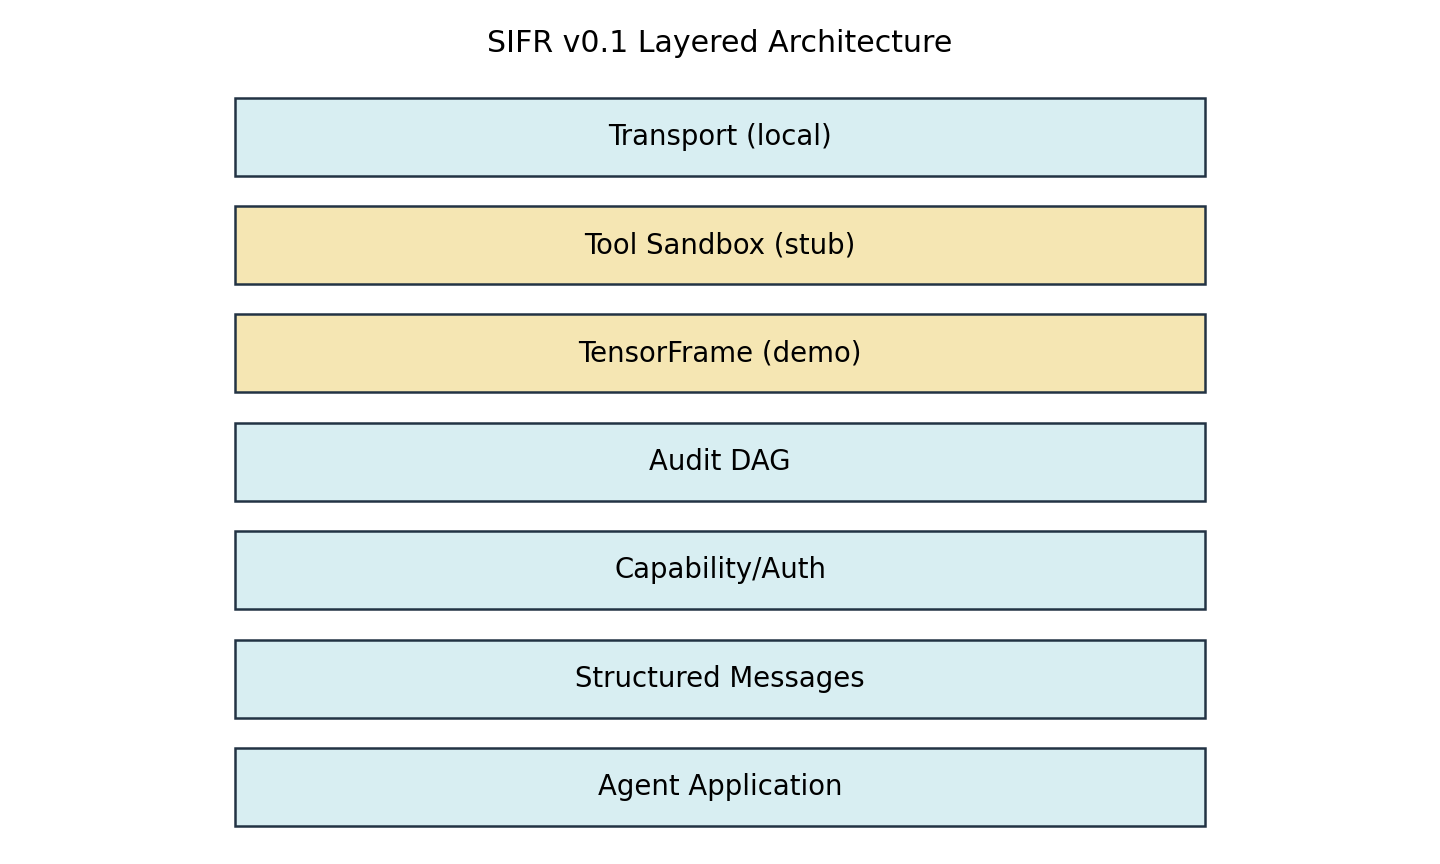
\includegraphics[width=\linewidth]{figures/architecture.png}
\caption{SIFR v0.1 layered architecture. Implemented layers are local and prototype-scoped; QUIC, WASM, DID/VC, and full interoperability are future work.}
\label{fig:architecture}
\end{figure}

\subsection{Message Envelope}
Every SIFR message contains a protocol version, message identifier, session identifier, type, sender identifier, receiver identifier, UTC timestamp, parent CIDs, optional capability identifier, payload, and optional signature. The signature is computed over the canonical message without the signature field. The implemented message types are Hello, CapabilityOffer, CapabilityGrant, Thought, Action, ToolUse, Observation, Result, Critique, Error, and TensorFrame.

\subsection{Canonicalization and Signatures}
The prototype canonicalizes messages by removing the signature field, sorting JSON keys, using compact JSON separators, and encoding UTF-8. Ed25519 signatures are generated and verified using the \texttt{cryptography} library. Verification fails if the payload, sender, or any signed field changes after signing.

\subsection{Capabilities}
A CapabilityGrant payload binds an issuer, subject, allowed actions, resource scope, issue time, expiration time, call budget, payload-size budget, and delegation constraint. The action verifier checks the grant signature, issuer consistency, subject match, action membership, expiration, payload size, call budget, and delegation policy before tool execution.

\subsection{Audit DAG}
Each accepted message can be added to an audit DAG. The CID is computed as SHA-256 over canonical message bytes without the signature field. Nodes record CID, message id, message type, sender, receiver, parents, timestamp, and signature-valid status. The DAG verifier detects missing parents, invalid signature flags, and stored-message mutation.

\begin{figure}[t]
\centering
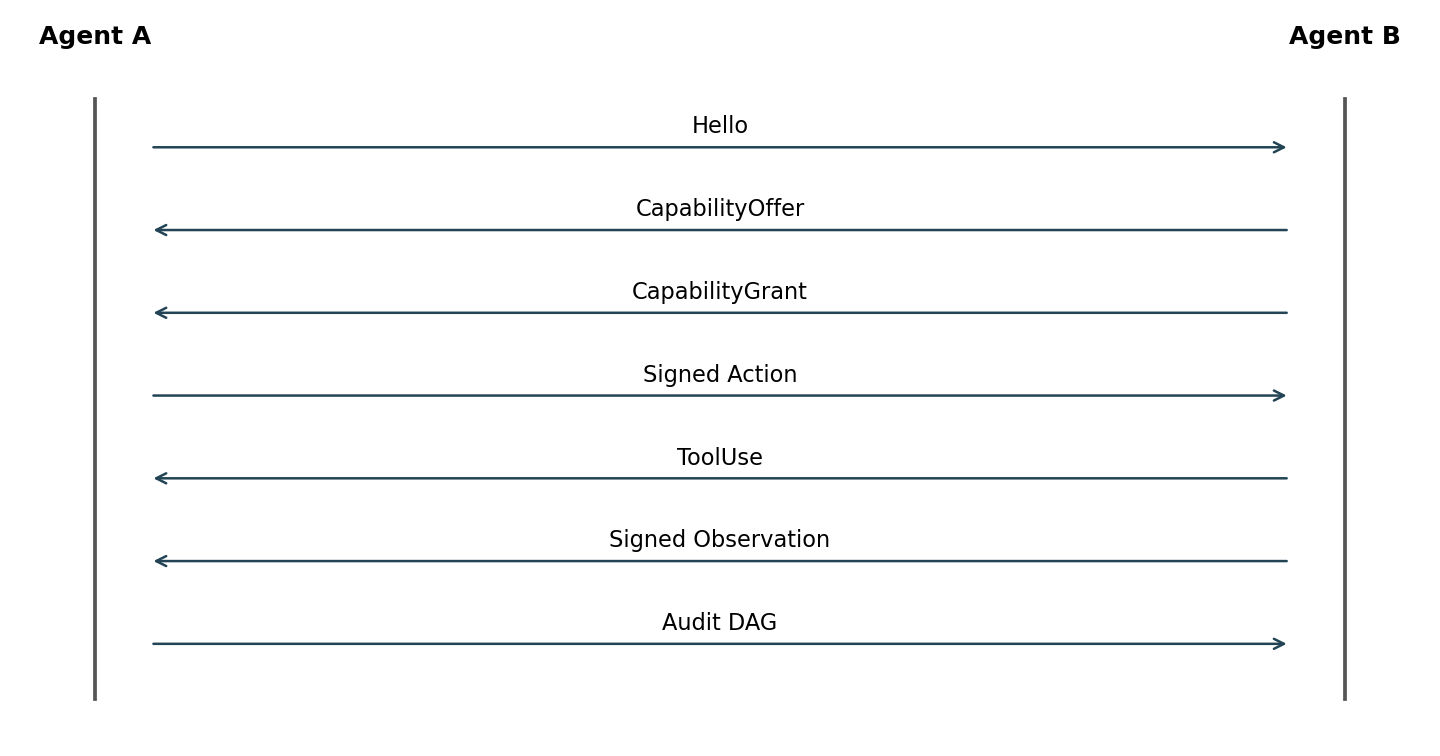
\includegraphics[width=\linewidth]{figures/handshake_sequence.png}
\caption{Two-agent SIFR v0.1 handshake and execution sequence.}
\label{fig:handshake}
\end{figure}

\begin{figure}[t]
\centering
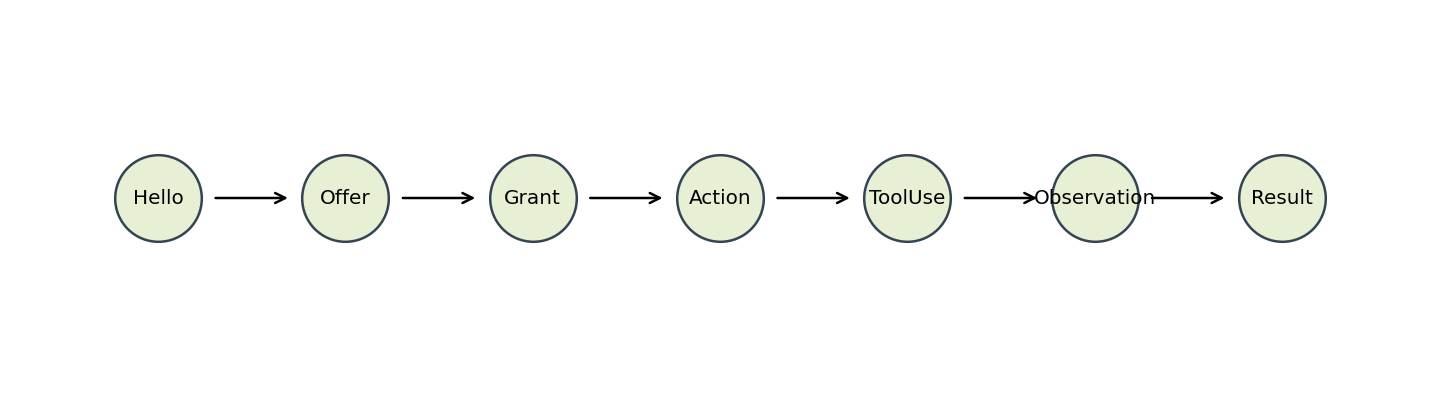
\includegraphics[width=\linewidth]{figures/audit_dag.png}
\caption{Audit DAG for the implemented vertical slice.}
\label{fig:dag}
\end{figure}

\section{Prototype Implementation}
The artifact is organized as a Python package with examples, tests, benchmarks, documentation, paper source, and review materials. Table~\ref{tab:implementation} summarizes the implementation status. The complete demo creates two agents: \texttt{did:sifr:planner} and \texttt{did:sifr:executor}. The planner sends a signed Hello. The executor sends a CapabilityOffer and a signed CapabilityGrant allowing \texttt{tool.calculator.add}. The planner sends a signed Action requesting addition of 2 and 3. The executor verifies the planner's signature, verifies the grant, enforces capability checks, records ToolUse, executes the calculator stub, returns a signed Observation, and verifies the resulting audit DAG.

\begin{table}[t]
\caption{Implementation Status}
\label{tab:implementation}
\centering
\begin{tabular}{lll}
\toprule
Component & Status & Evidence\\
\midrule
Typed envelope & Implemented & \texttt{sifr/messages.py}\\
Ed25519 signing & Implemented & \texttt{sifr/crypto.py}\\
Capability grants & Implemented & \texttt{sifr/capabilities.py}\\
Audit DAG & Implemented & \texttt{sifr/audit\_dag.py}\\
Local transport & Implemented & \texttt{sifr/transport.py}\\
TensorFrame encoding & Demo & \texttt{sifr/tensor.py}\\
Calculator tool & Stub & \texttt{sifr/wasm\_runner.py}\\
QUIC backend & Future & Not implemented\\
WASM isolation & Future & Not implemented\\
DID/VC stack & Future & Syntax only\\
\bottomrule
\end{tabular}
\end{table}

\section{Security Model and Threat Analysis}
SIFR v0.1 assumes that each verifier already has the correct public key for the relevant agent. This is a significant limitation: the prototype tests frame integrity and capability enforcement, not production identity discovery. The security-oriented prototype goal is to reject tampered frames, unsigned frames, wrong-key verification, expired grants, wrong-subject grants, unauthorized actions, over-budget actions, and simple audit-DAG mutation.

Listing~\ref{lst:verify} summarizes the implemented verifier logic. The key point is that signature verification and capability authorization are separate checks: a correctly signed Action can still be rejected if it lacks the right grant.

\begin{lstlisting}[caption={Capability and DAG verification sketch for SIFR v0.1.},label={lst:verify}]
authorize(action, grant, issuer_pubkey, store):
  verify_signature(action, sender_pubkey)
  verify_signature(grant, issuer_pubkey)
  require grant.payload.issuer == grant.sender_id
  require action.capability_id == grant.capability_id
  require grant.subject == action.sender_id
  require action.payload.action in grant.actions
  require now_utc < grant.expires_at
  require size(action.payload) <= grant.max_payload_bytes
  require store.calls(grant.id) < grant.max_calls
  require not action.delegate_to or grant.allow_delegation
  store.consume(grant.id)
  return ALLOW

verify_dag(dag):
  for node in dag.nodes:
    require sha256(canonical(node.message)) == node.cid
    require node.signature_valid
    for parent in node.parents:
      require parent in dag.nodes
  return OK
\end{lstlisting}

\begin{table}[t]
\caption{Threat Handling in SIFR v0.1}
\label{tab:threats}
\centering
\begin{tabular}{lll}
\toprule
Threat & v0.1 Mechanism & Status\\
\midrule
Payload tampering & Ed25519 verify & Tested\\
Sender tampering & Signed sender field & Tested\\
Wrong key & Public-key verify failure & Tested\\
Unsigned message & Signature required & Tested\\
Unauthorized action & Capability action check & Tested\\
Wrong subject & Capability subject check & Tested\\
Expired grant & UTC expiration check & Tested\\
Over budget & Call counter & Tested\\
DAG mutation & CID recomputation & Tested\\
Missing parent & Parent lookup & Tested\\
Replay & Message IDs only & Future\\
Revocation & None & Future\\
Prompt injection & Out of scope & Future\\
Sandbox escape & Stub only & Future\\
\bottomrule
\end{tabular}
\end{table}

The prototype deliberately does not claim formal security. Signatures establish message integrity under the assumed public key, but do not establish trust by themselves. Capability grants authorize specific actions, but v0.1 lacks revocation, distributed state, concurrent budget reservations, and replay protection. The calculator tool is bounded because it performs only a structured addition operation; it is not evidence that arbitrary generated code can be safely executed.

\section{Evaluation}
\subsection{Experimental Setup}
All measurements were generated by the included scripts under \texttt{benchmarks/}. The environment metadata is stored in \texttt{benchmarks/results/environment.json}. The current raw results were generated on Windows with Python 3.14.2. The benchmarks are local microbenchmarks and should not be interpreted as distributed network performance.

\subsection{Payload Size}
Table~\ref{tab:payload} and Figure~\ref{fig:payload} compare a plain JSON action, unsigned SIFR action, signed SIFR action, TensorFrame JSON-list encoding, and TensorFrame base64 binary encoding. The signed SIFR frame is larger than a plain JSON action because it carries versioning, identifiers, parents, sender/receiver identifiers, timestamp, capability id, and signature. For the tested 384-dimensional float32 vector, base64 binary encoding is substantially smaller than a JSON float list.

\begin{table}[t]
\caption{Payload Size Benchmark}
\label{tab:payload}
\centering
\begin{tabular}{lrr}
\toprule
Case & Bytes & Ratio vs. plain\\
\midrule
Plain JSON action & 53 & 1.00\\
SIFR unsigned action & 257 & 4.85\\
SIFR signed action & 411 & 7.75\\
Tensor JSON list & 7642 & 144.19\\
Tensor base64 binary & 2214 & 41.77\\
\bottomrule
\end{tabular}
\end{table}

\begin{figure}[t]
\centering
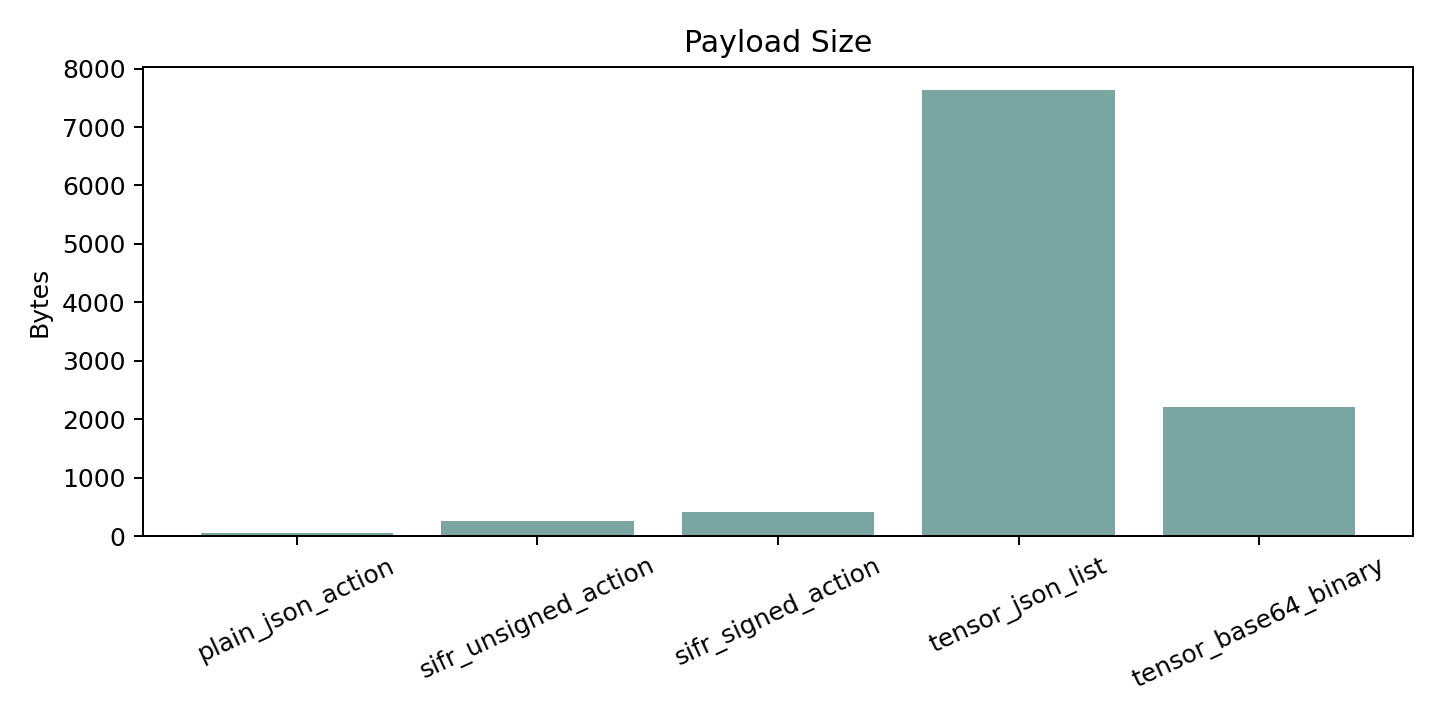
\includegraphics[width=\linewidth]{figures/benchmark_payload.png}
\caption{Payload-size benchmark generated from raw CSV results.}
\label{fig:payload}
\end{figure}

\subsection{Signature Overhead}
The Ed25519 microbenchmark creates, signs, and verifies 100, 1000, and 10000 messages. At 10000 messages, average signing time was 0.0314 ms per message and average verification time was 0.0615 ms per message. Figure~\ref{fig:signature} plots average cost across message counts. These measurements support H4 only for local CPU overhead, not for networked deployment.

\begin{figure}[t]
\centering
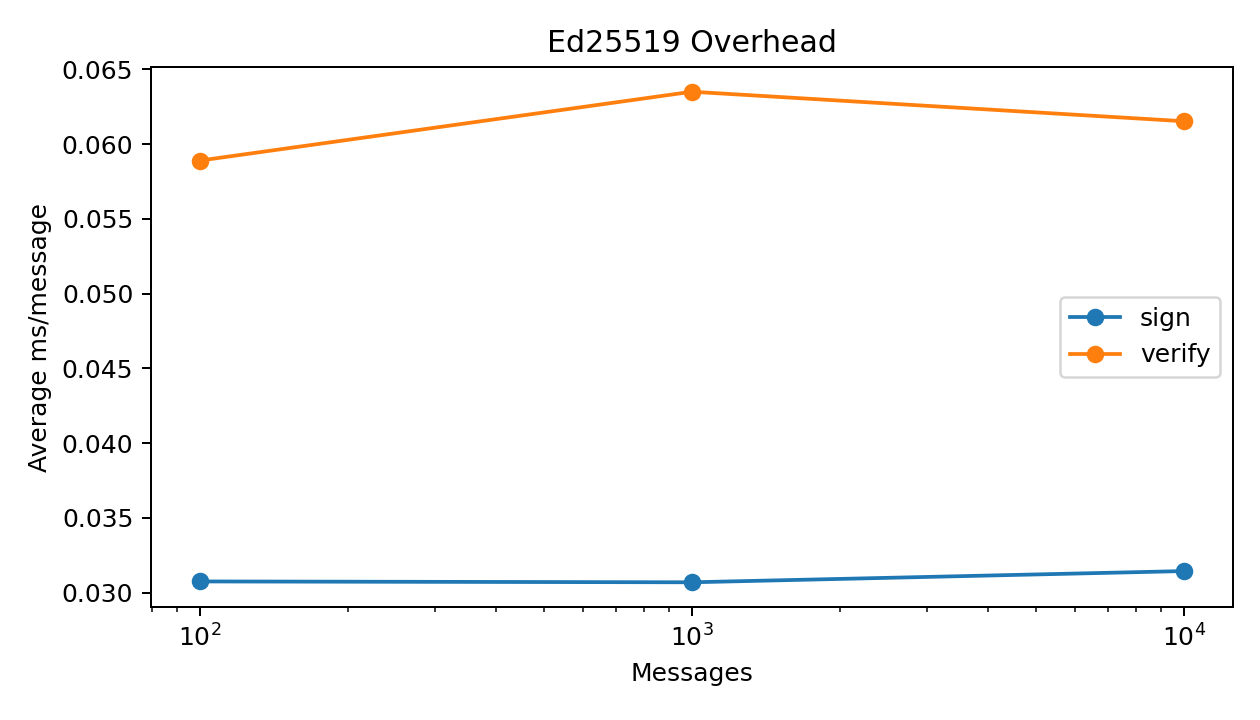
\includegraphics[width=\linewidth]{figures/benchmark_signature_overhead.png}
\caption{Ed25519 signing and verification overhead.}
\label{fig:signature}
\end{figure}

\subsection{Latency}
The latency benchmark compares plain local dict passing, SIFR message creation, SIFR signing plus verification, SIFR signing plus verification plus DAG append, and JSON serialization/deserialization as a simulated HTTP JSON baseline. Table~\ref{tab:latency} and Figure~\ref{fig:latency} report local latency only.

\begin{table}[t]
\caption{Local Latency Microbenchmark}
\label{tab:latency}
\centering
\begin{tabular}{lrr}
\toprule
Case & Mean ms & p95 ms\\
\midrule
Plain local dict & 0.00017 & 0.00040\\
SIFR create only & 0.00779 & 0.01810\\
SIFR sign+verify & 0.09833 & 0.12360\\
SIFR sign+verify+DAG & 0.11040 & 0.15260\\
HTTP JSON serialization & 0.00758 & 0.01360\\
\bottomrule
\end{tabular}
\end{table}

\begin{figure}[t]
\centering
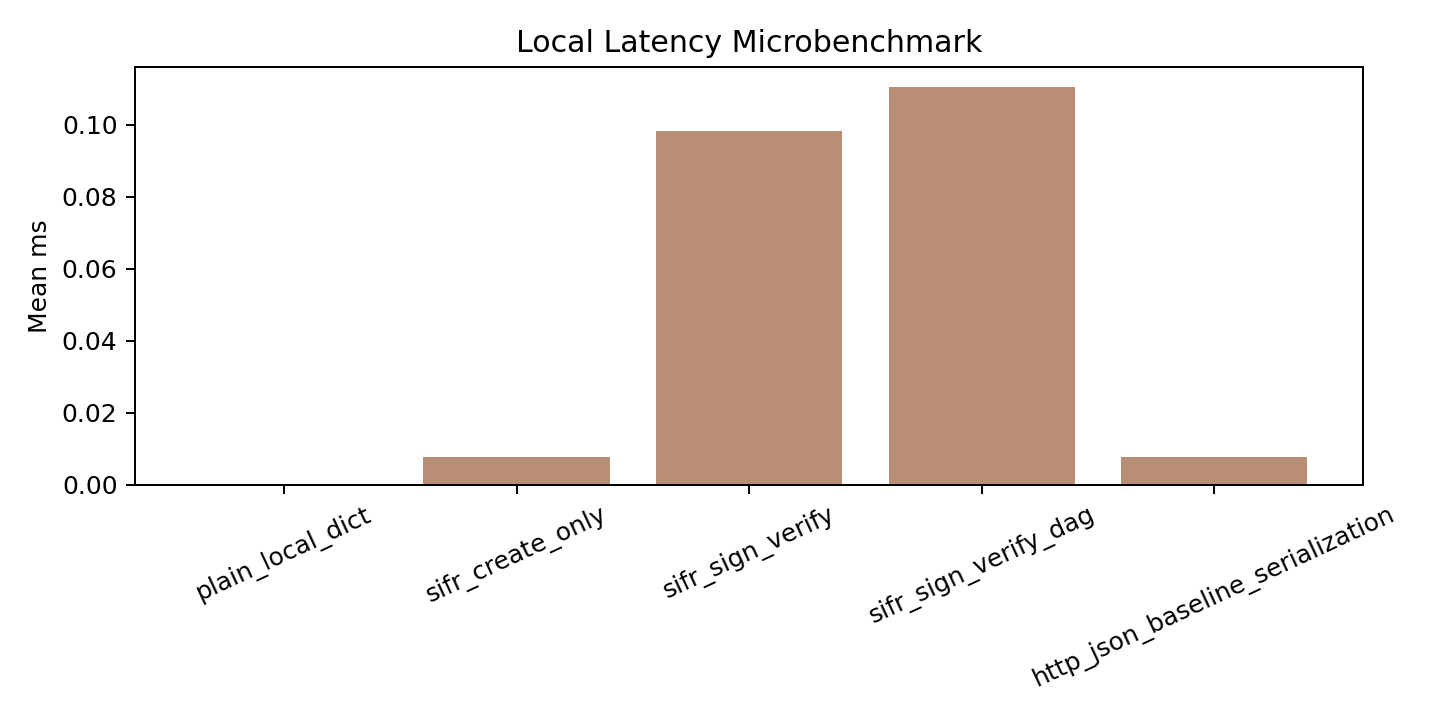
\includegraphics[width=\linewidth]{figures/benchmark_latency.png}
\caption{Local latency microbenchmark.}
\label{fig:latency}
\end{figure}

\subsection{Capability Enforcement}
The capability benchmark runs six cases: authorized action, unauthorized action, expired capability, tampered capability, over-budget capability, and wrong subject. The authorized action succeeds. The remaining five cases are rejected with the expected error category. This supports H2 for the implemented two-agent calculator workflow.

\begin{figure}[t]
\centering
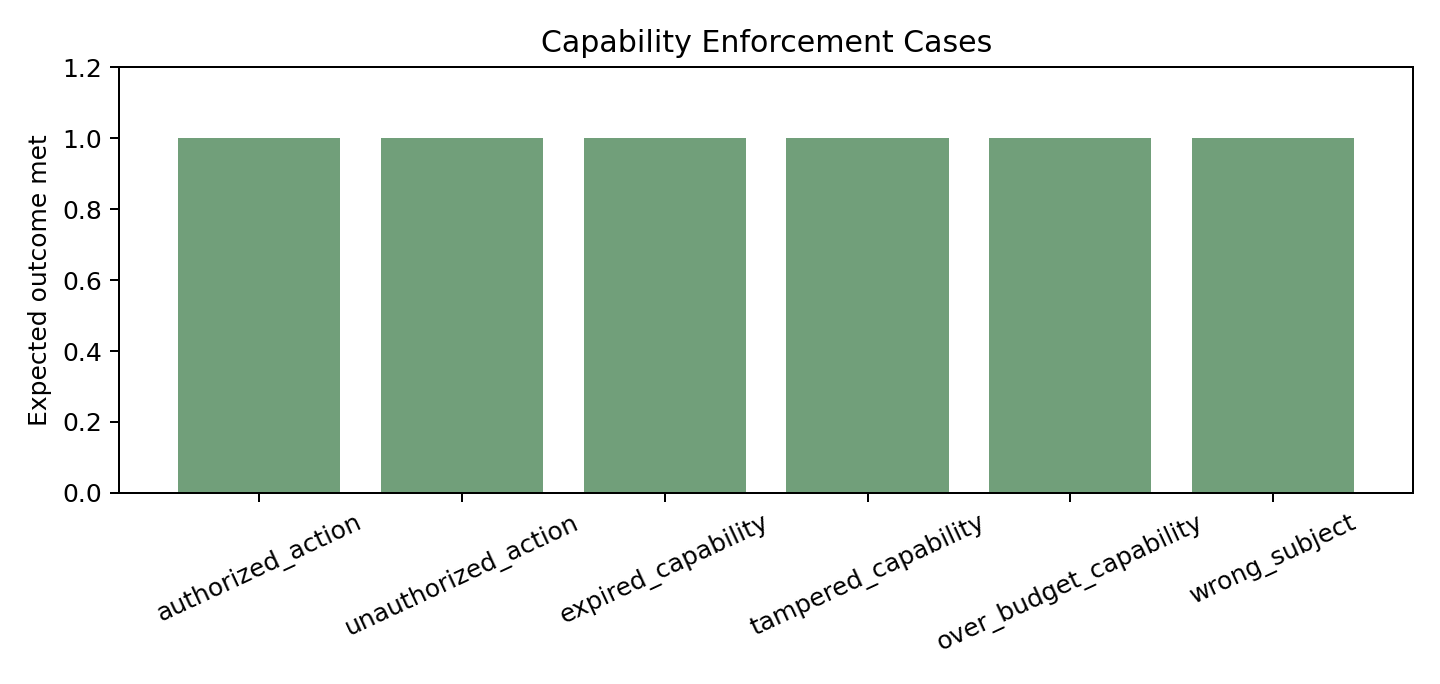
\includegraphics[width=\linewidth]{figures/benchmark_capability.png}
\caption{Capability-enforcement benchmark. The authorized case succeeds; negative cases are expected rejections.}
\label{fig:capability}
\end{figure}

\section{Discussion}
The prototype demonstrates that a compact vertical slice can bind communication semantics, signatures, capabilities, tool execution, and audit lineage. This is the main value of SIFR v0.1: not that the protocol is complete, but that the implementation makes a research claim testable. A reviewer can run the demo, tamper with frames, expire grants, exceed budgets, remove DAG parents, regenerate figures, and inspect the resulting behavior.

The results also show costs and trade-offs. Signed frames are larger than plain JSON actions. Ed25519 verification is slower than signing in the measured environment. DAG append adds additional local overhead. These costs may be acceptable for integrity-sensitive agent workflows, but the current evaluation is too small to justify broad performance claims. The TensorFrame experiment demonstrates encoding-size differences only; it does not demonstrate privacy, semantic quality, compression efficiency, or safe KV-cache sharing.

\section{Limitations}
SIFR v0.1 is an early research prototype. It does not include a QUIC backend, WASM/WASI isolation, DID resolution, Verifiable Credential issuance or verification, grant revocation, replay cache, distributed log consensus, formal verification, fuzzing, or network adversary testing. Capability budgets are stored in a local in-memory counter and are not atomic across distributed processes. The audit DAG detects mutation of stored accepted messages, but v0.1 does not log all malformed or rejected probes. Public-key distribution is assumed out of band. The paper therefore should be read as an early feasibility artifact, not a production protocol specification.

\section{Future Work}
Future work should implement QUIC transport and compare local, loopback, and networked latency; add replay caches and revocation; integrate a real DID/VC trust layer; replace the calculator stub with WASM/WASI sandboxed tools; add MCP, A2A, ACP, ANP, and HTTP JSON adapters; log denied and malformed requests in the audit layer; implement concurrency-safe budget reservation; add fuzzing and property-based tests; and study privacy-preserving TensorFrame designs in light of embedding inversion and KV-cache leakage research.

\section{Conclusion}
SIFR v0.1 proposes and implements a narrow but complete vertical slice for structured, signed, capability-checked AI-agent communication. The prototype shows that Hello, capability negotiation, signed authorization, bounded tool execution, signed observation, and audit-DAG verification can be integrated into a reproducible research artifact. The measured local overhead is concrete: a signed SIFR action is 411 bytes versus 53 bytes for plain JSON, signing averages 0.0314 ms, verification averages 0.0615 ms, and sign+verify+DAG latency averages 0.1104 ms in the current environment. The work is deliberately scoped and not production-ready, but it provides a concrete baseline for future agent-native protocol research.

\section*{Reproducibility Statement}
The artifact includes source code, tests, benchmark scripts, raw benchmark files, generated plots, paper source, and review notes. From the repository root, run:
\begin{verbatim}
pip install -r requirements.txt
pytest
python examples/demo_two_agents.py
bash scripts/run_benchmarks.sh
python scripts/generate_figures.py
\end{verbatim}
On Windows without Bash, run each Python benchmark script directly. The Overleaf-ready paper is in the \texttt{paper/} directory.

\bibliographystyle{IEEEtran}
\bibliography{references}

\end{document}
